% -------------- PREÁMBULO SUGERIDO --------------
\documentclass[12pt]{article}
\usepackage{babel}
\usepackage[utf8]{inputenc}
\usepackage[T1]{fontenc}
\usepackage{lmodern}
\usepackage{amsmath, amssymb}
\usepackage{graphicx}
\usepackage{float}
\graphicspath{{figs/}}    % nueva línea
\usepackage{booktabs}
\usepackage{hyperref}
\usepackage{geometry}
\geometry{margin=2.5cm}
% -----------------------------------------------

\begin{document}

\title{Lección 22:\\ Leyes de Kepler, Órbitas Elípticas y Cambio de Órbitas}
\author{Walter Lewin — 8.01 Física I: Mecánica Clásica, 1999\\
(Massachusetts Institute of Technology: MIT OpenCourseWare)\\
\href{http://ocw.mit.edu}{ocw.mit.edu} (consultado 08/04/2013)\\
Licencia CC BY-NC-SA}
\date{}
\maketitle


\section{Leyes de Kepler y órbitas elípticas}

\subsection{Repaso: órbita circular}

Un objeto de masa $m$ gira alrededor de $M$ (Fig.~\ref{fig:circulo}).

\begin{figure}[h]
  \centering
  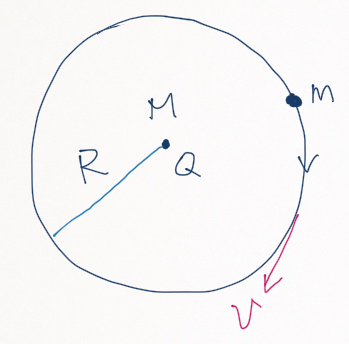
\includegraphics[width=0.55\textwidth]{01.png}
  \caption{Órbita circular.}
  \label{fig:circulo}
\end{figure}

\begin{enumerate}
  \item \[
    T^{2} = \frac{4\pi^{2}R^{3}}{GM}
  \]

  \item \[
    v = \frac{2\pi R}{T} = \sqrt{\frac{GM}{R}}
  \]

  \item \[
    E_{\text{tot}} = \frac12 m v^{2}-\frac{mGM}{R}
      = -\frac{mGM}{2R}
  \]

  \item \[
    v_{\text{escape}} = \sqrt{2}\,v = \sqrt{\frac{2GM}{R}}
  \]
\end{enumerate}

Cerca de la Tierra: $T\!\approx\!90$ min, $v\!\approx\!8$ km/s y $v_{\text{escape}}\!\approx\!11{,}2$ km/s.  
La Tierra alrededor del Sol: $T\!\approx\!365$ días, $v\!\approx\!30$ km/s.

\subsection{Las tres leyes de Kepler}

\begin{enumerate}
  \item Las órbitas son elipses con el Sol en un foco.
  \item Áreas iguales en tiempos iguales (Fig.~\ref{fig:areas}).
  \item $T^{2}\propto (\text{distancia media})^{3}$.
\end{enumerate}

\begin{figure}[h]
  \centering
  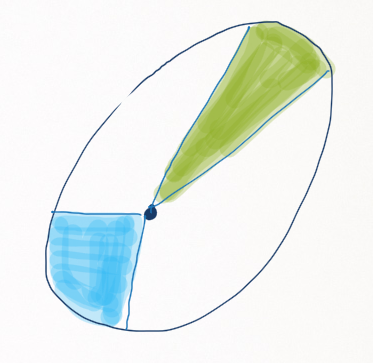
\includegraphics[width=0.55\textwidth]{02.png}
  \caption{Áreas iguales en tiempos iguales.}
  \label{fig:areas}
\end{figure}

\paragraph{Datos que usó Kepler (1618).}

\begin{table}[h]
\centering
\begin{tabular}{@{}l c c c@{}}
\toprule
Planeta &
$R$ (UA) &
$T$ (días) &
\parbox[c]{3.2cm}{\centering $R^{3}/T^{2}$\\($10^{-6}$ UA$^{3}$/día$^{2}$)}\\
\midrule
Mercurio & 0.389 &  87.77  & 7.64\\
Venus    & 0.724 & 224.70  & 7.52\\
Tierra   & 1.000 & 365.25  & 7.50\\
Marte    & 1.524 & 686.98  & 7.50\\
Júpiter  & 5.200 & 4\,332.62 & 7.49\\
Saturno  & 9.510 & 10\,759.2 & 7.43\\
\bottomrule
\end{tabular}
\caption{Constancia de $R^{3}/T^{2}$ en los planetas conocidos.}
\end{table}

\subsection{Propiedades de la órbita elíptica}

\begin{figure}[h]
  \centering
  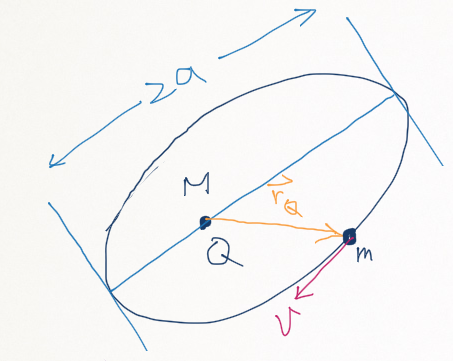
\includegraphics[width=0.55\textwidth]{03.png}
  \caption{Elementos de una elipse orbital.}
\end{figure}

Para una elipse de semieje mayor $a$:
\[
E_{\text{tot}} = \frac12 m v^{2}-\frac{mGM}{r} = -\frac{mGM}{2a},
\qquad
T^{2} = \frac{4\pi^{2}a^{3}}{GM}.
\]

Órbitas con el mismo $a$ comparten idéntico periodo y energía total (Fig.~\ref{fig:mismoa}).

\begin{figure}[h]
  \centering
  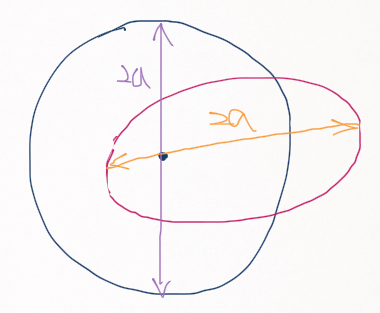
\includegraphics[width=0.55\textwidth]{04.png}
  \caption{Mismo $a$ $\Rightarrow$ mismo $T$ y $E$.}
  \label{fig:mismoa}
\end{figure}

\section{Órbita elíptica a partir de condiciones iniciales}

\begin{figure}[h]
  \centering
  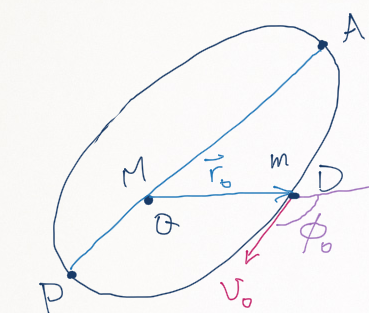
\includegraphics[width=0.55\textwidth]{05.png}
  \caption{Geometría para obtener los parámetros orbitales.}
\end{figure}

Condiciones iniciales $(M,\,v_0,\,\mathbf r_0,\,\phi_0)$:
\[
a = \frac{GM\,r_0}{r_0 v_0^{2}-2GM}.
\]

\noindent
Luego $T$ se halla con la 3.ª ley de Kepler.  
Conservación del momento angular sobre $Q$:
\[
m v_0 r_0\sin\phi_0 = m v_P\,QP = m v_A\,QA.
\]

\paragraph{Ejemplo numérico.}
\[
M=6{\times}10^{24}\,\text{kg},\;
r_0=9000\,\text{km},\;
v_0=9.0\,\text{km/s},\;
\phi_0=120^{\circ}
\]
\[
a\approx50\,000\,\text{km},\;
T\approx31\,\text{h},\;
QP\approx6.6{\times}10^{3}\,\text{km},\;
v_P\approx10.7\,\text{km/s}.
\]

\section{Cambiar de órbita circular a elíptica}

\begin{figure}[h]
  \centering
  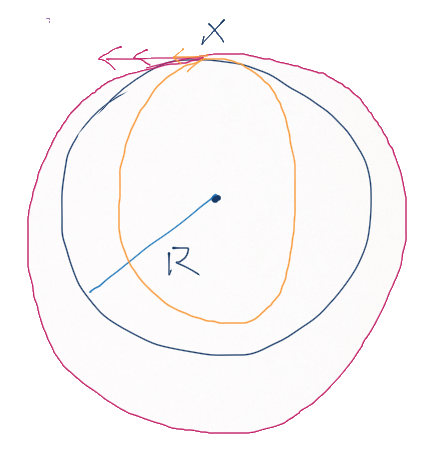
\includegraphics[width=0.55\textwidth]{06.png}
  \caption{Efecto de un \(\Delta v\) tangencial en \(X\).}
\end{figure}

\begin{itemize}
\item \textbf{Impulso progrado} ($\Delta v>0$): $E_{\text{tot}}\!\uparrow\!\Rightarrow 2a>2R$, $T>T_{\text{circ}}$.
\item \textbf{Impulso retrógrado} ($\Delta v<0$): $E_{\text{tot}}\!\downarrow\!\Rightarrow 2a<2R$, $T<T_{\text{circ}}$.
\end{itemize}

\section{Dos astronautas y un sándwich}

\begin{figure}[h]
  \centering
  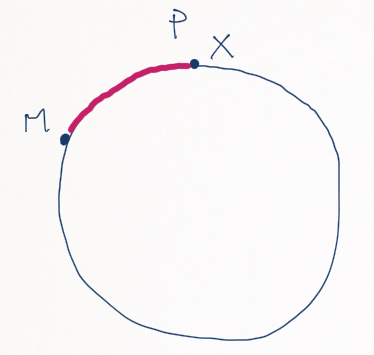
\includegraphics[width=0.55\textwidth]{07.png}
  \caption{Pedro (rojo) quiere lanzar un sándwich a María (amarillo).}
\end{figure}

Separados por un arco $f\,2\pi R$, se desea que el periodo del sándwich cumpla
\[
T_s = (1-f)\,T_a \;\Longrightarrow\;
a = R\,(1-f)^{2/3}.
\]

Generalizando con $n_a$ y $n_s$ vueltas:
\[
a = R\!\left(\frac{n_a-f}{n_s}\right)^{2/3},\qquad
\Delta v = v_s-v_a.
\]

\paragraph{Ejemplo.}  
$R=7000$ km, $f=0.05$:
\[
a = 6765\,\text{km},\;
v_s = 7.42\,\text{km/s},\;
\Delta v = -0.13\,\text{km/s}.
\]

\subsection*{¿Atrapar o no atrapar?}

\begin{table}[h]
\centering
\begin{tabular}{@{}ccccl@{}}
\toprule
$f$ & $n_a$ & $n_s$ & $(v_s-v_a)/v_a$ & Resultado\\
\midrule
0.05 & 1 & 1 & $-0.01755$ & re-entrada\\
0.05 & 1 & 2 & $-0.402$   & re-entrada\\
0.05 & 1 & 3 & sin solución & ($a<R/2$)\\
0.05 & — & — & $-1.0$ & caída radial\\
0.05 & 1 & 1 & $-0.01755$ & \textbf{atrapa}\\
0.05 & — & — & $+0.164$ & casi llega\\
0.05 & — & — & $+0.42$  & ¡escapa!\\
\bottomrule
\end{tabular}
\caption{Algunos escenarios para el lanzamiento del sándwich.}
\end{table}

\begin{figure}[h]
  \centering
  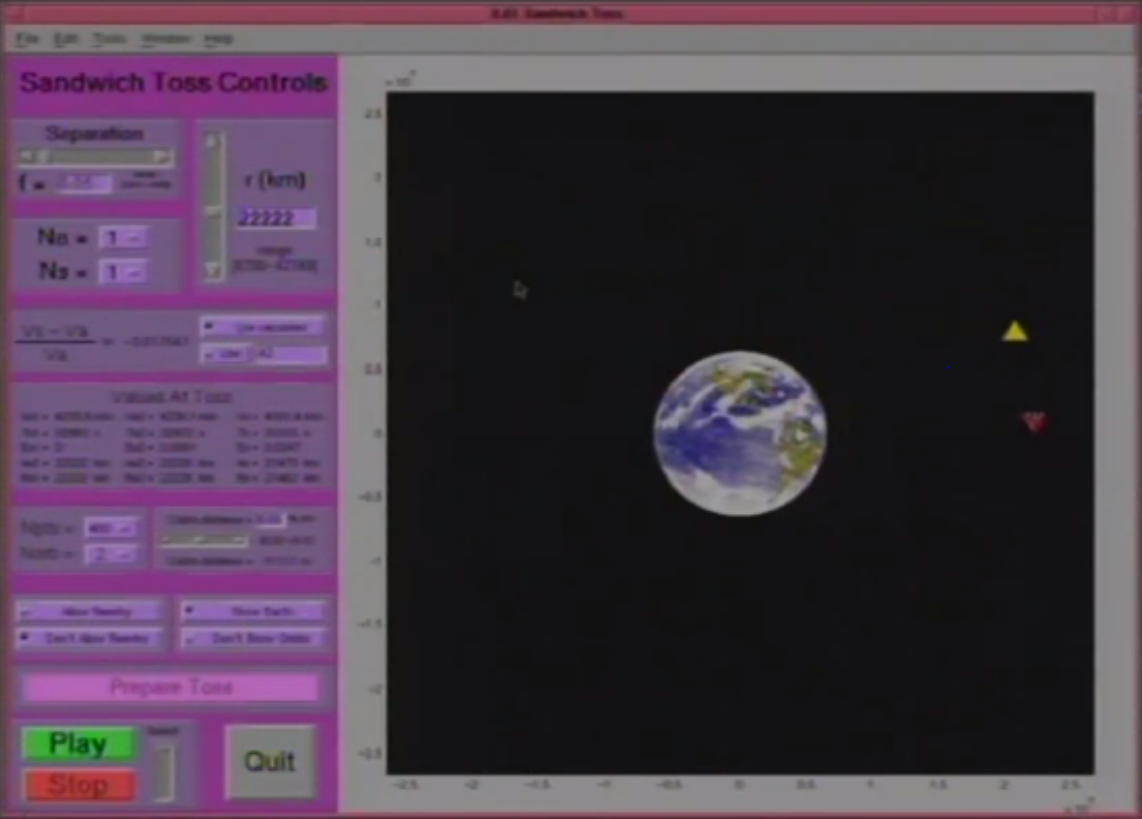
\includegraphics[width=0.55\textwidth]{08.png}
  \caption{Simulación por computadora de varios lanzamientos.}
\end{figure}

\end{document}
